% ch-ref-domain.tex -- reference: root keys, Grid, Initial, Substrate, Fluid
\chapter{格子、初期状態、基板、流体}
\label{ch:ref-domain}

本章では、\emph{何を}計算するかを定める四つのブロックを説明する。格子と計算領域
（\key{Grid}）、計算開始時の状態（\key{Initial}）、液膜の下にある固体の形状
（\key{Substrate}）、液体の物性値（\key{Fluid}）である。どのブロックにも属さず
ルートレベルに置く少数のキーもあわせて扱う。物理項、境界条件、数値計算の設定は
\cref{ch:ref-physics,ch:ref-bcout,ch:ref-numerics}で述べる。

本章に示す既定値、型、範囲は、いずれもパーサーが実際に適用する値である。
\reqd{}と記したキーを省略すると、計算は終了する。\emph{範囲 $[a:b]$}と書いた範囲や
\emph{以上}と書いた下限は、ファイルの読み込み時に検査する。範囲を外れた値があると
計算は止まる。一方、\emph{正}や\emph{非ゼロ}といった語は意味のある値の目安であり、
検査はしない。これらの表とパーサーの一致は\file{tools/doc\_keys.py}で確認しており、
\code{ctest}がこれを実行する（\code{doc\_keys}）。

\section{ルートレベル}
\label{sec:ref-domain:root}

ファイルの先頭、最初のテーブルヘッダーより前に書くキーは、計算の識別と水平方向の
長さスケールの選択に使う。\key{SolverName}はバージョンの確認用であり、ソルバーを選ぶ
キーではない。モデルは\key{Physics.ConcField.Model}と\key{Grid.Dimension}の組合せで決まる。
\key{JobName}は、実行した場所に作る結果ディレクトリの名前である。入力ファイルは
そこへコピーされ、ParaViewのインデックスファイルにもこの名前が付く。

\begin{keytable}{ルートレベルのキー\label{tab:root-keys}}\key{SolverName} & string & \reqd & ソルバーと入力形式の識別子。\val{"Yuzen-1.0"}と完全に一致しなければならず、ほかの文字列では計算を中止する。\code{MAJOR.MINOR}の系列だけを表すので、パッチリリースでは変わらない（\cref{ch:policy}）。 \\
\key{JobName} & string & \reqd & 結果ディレクトリの名前。任意の文字列。 \\
\key{LengthScaleType} & string & \val{"capillary"} & 水平方向の長さスケール$L_0$の決め方。\val{"capillary"}なら$L_0=\sqrt{\sigma_0/(\rho g)}$、\val{"custom"}なら\key{LengthScale}の値を$L_0$とする。 \\
\key{LengthScale} & double & \val{1.0} & 水平方向の長さスケール（メートル）。常に読み込むが、使うのは\key{LengthScaleType}が\val{"custom"}のときだけである。実用上は正。 \\
\key{InputFormatVersion} & string & \val{"1.0"} & ファイルが前提とする入力形式のバージョン。指定する場合は\val{"1.0"}とする。本バージョンが読めるのはこの形式だけである（\cref{sec:ref-numerics:formatversion}）。 \\
\end{keytable}

\file{cases/}のケースはどれも長さスケールのキーを設定していない。したがって、同梱の
ケースはすべて毛管長を長さスケールとして計算する。

\section{\key{Grid}}
\label{sec:ref-domain:grid}

\key{Grid}は必須であり、ちょうど一回だけ書く。重複すると計算を中止する。
このブロックでは、問題の次元、内部セルの数、計算領域の物理的な大きさを定める。
内部では各辺に二層のゴーストセルを加えるので、ソルバーが確保する配列は
\key{Nx}と\key{Ny}から想像するより大きい。

\begin{keytable}{\key{Grid}のキー\label{tab:grid-keys}}\key{Dimension} & string & \reqd & \val{"xh"}は水平一方向（1次元の液膜）、\val{"xyh"}は水平二方向。\key{Physics.ConcField.Model}との組合せでソルバーのモデルが決まる。 \\
\key{Nx} & int & \reqd & $x$方向のセル数。範囲 $[1:1000000]$。 \\
\key{Ny} & int & \val{1} & $y$方向のセル数。範囲 $[1:1000000]$。\key{Dimension}が\val{"xyh"}のときは$\ge 2$とする。\val{"xh"}では液膜は1次元であり、\key{Ny}は使わない。ただし\val{"CZ"}モデルはこの値を読み、1以外が設定されていれば警告を出して1に戻す。 \\
\key{Nz} & int & \val{1} & 膜厚方向のセル数。範囲 $[1:1000000]$。使うのは\val{"CZ"}モデルだけで、$\mathrm{Nz}\ge 2$を要求する。鉛直一様モデルではどれも無視する。 \\
\key{Xmin} & double & \reqd & 計算領域の$x$の下限（メートル）。 \\
\key{Xmax} & double & \reqd & $x$の上限（メートル）。\key{Xmin}より大きい値とする。セル幅は$(\mathrm{Xmax}-\mathrm{Xmin})/\mathrm{Nx}$である。 \\
\key{Ymin} & double & \val{0} & $y$の下限（メートル）。\key{Dimension}が\val{"xh"}のときは、読み込むが使わない。 \\
\key{Ymax} & double & \val{1} & $y$の上限（メートル）。\key{Dimension}が\val{"xh"}のときは、読み込むが使わない。 \\
\end{keytable}

\begin{note}[軸ごとの上限のほかに総数の上限もある]
  セル数の上限は軸ごとに百万であるが、その積にも上限がある。
  $(\mathrm{Nx}+4)(\mathrm{Ny}+4)(\mathrm{Nz}+4)$は$5\times10^{7}$以下とし、
  これを超えるファイルは範囲エラーとして拒否する。格子の線形インデックスが
  \code{int}型であるためで、この上限があればインデックスは型の範囲に十分収まる。
  もう一つの制約はメモリである。鉛直一様モデルで$1024^{2}$の液膜を計算するには約
  \SI{4}{\giga\byte}が必要であり、2次元での上限（約$10^{7}$セル）では約
  \SI{40}{\giga\byte}になる。1ステップに必要なメモリは、2次元ではセルあたり約
  \SI{4}{\kilo\byte}、1次元では\SI{2}{\kilo\byte}、\val{"CZ"}では
  $\mathrm{Nx}\,\mathrm{Ny}\,\mathrm{Nz}$のセルあたり\SI{2}{\kilo\byte}である
  （\cref{sec:verification:long}）。
\end{note}

\begin{note}[使わない$y$の範囲はエラーにならない]
  \val{"xh"}の計算では、$y$の範囲は読み込んだうえで無視する。そのため、同じケースの2次元版の
  値が残っていても何も警告は出ない。\file{cases/allphys\_1d\_reg.toml}がその例であり、
  \key{Ymin} $=-1$、\key{Ymax} $=1$メートルとなっている。こうした値を
  計算領域の指定と受け取ってはならない。
\end{note}

\section{\key{Initial}}
\label{sec:ref-domain:initial}

\key{Initial}は必須で、ちょうど一回だけ書く。このブロック自身のキーはない。
\key{Concentration}と\key{SurfaceShape}をまとめる入れ物であり、この二つもそれぞれ必須である。
両者で$t=0$の液膜を定める。\key{Restart.Enable}が真のときは、リスタートファイルで
置き換えられる状態を定めることになる。

\subsection{\key{Initial.Concentration}}

\begin{keytable}{\key{Initial.Concentration}のキー\label{tab:initial-conc-keys}}\key{Value} & double & \reqd & 溶質（樹脂）の初期濃度。質量分率で、範囲 $[0:1]$。この値をすべてのセルに設定する。 \\
\key{Type} & string & \val{"uniform"} & 初期濃度場の形。選べるのは\val{"uniform"}だけであり、ほかの文字列では計算を中止する。 \\
\end{keytable}

\subsection{\key{Initial.SurfaceShape}}

このブロックでは、問題全体の膜厚スケールと前駆膜を設定する。膜厚分布を組み立てる形状ブロックも
この中に書く。

\begin{keytable}{\key{Initial.SurfaceShape}のキー\label{tab:initial-shape-keys}}\key{TotalHeight} & double & \val{1} & 膜厚スケール$h_0$（メートル）。正。以下の形状はすべてこの値に掛ける無次元の倍率である。無次元化（$T_0$、$\As$、$\Ev$、$\Df$、$\Spn$）もすべてこの値をもとにする。 \\
\key{PrecursorRatio} & double & \val{0} & 前駆膜の厚さと\key{TotalHeight}の比（無次元比$\Hstar$）。実用上は$[0:1)$。\key{Physics.DisjoiningPressure.Enable}が真のときは$>0$とする必要があり、そうでなければ計算を中止する。非ゼロにすると、蒸発速度の薄膜補正も有効になる。 \\
\end{keytable}

膜厚の分布は次のように組み立てる。
\[
  h = \mathrm{TotalHeight}\,\bigl(\text{shape}\cdot(1-\Hstar) + \Hstar\bigr),
\]
ここから基板形状を差し引く。その際、液膜が前駆膜より薄く
ならないよう、$\hstar = \Hstar\cdot\mathrm{TotalHeight}$を下限とする。

\subsection{七つの形状}
\label{sec:ref-domain:shapes}

\key{Initial.SurfaceShape}の中では七つの形状ブロックを使える。\textbf{どれも何回でも
繰り返してよく}、一度も使わなくてもよい。各形状を\cref{fig:shapes-1d}に示す。式を読む前に
この図を参照されたい。以下の小節では各形状の定義とキーを示すが、\key{SmoothConvex}と
\key{MexicanHat}のどちらを選ぶか判断したり、\key{FlatPlane}が段差ではなく傾いた平面で
あることを確かめたりするには、図を見るのが最も早い。

\begin{figure}[tbp]
  \centering
  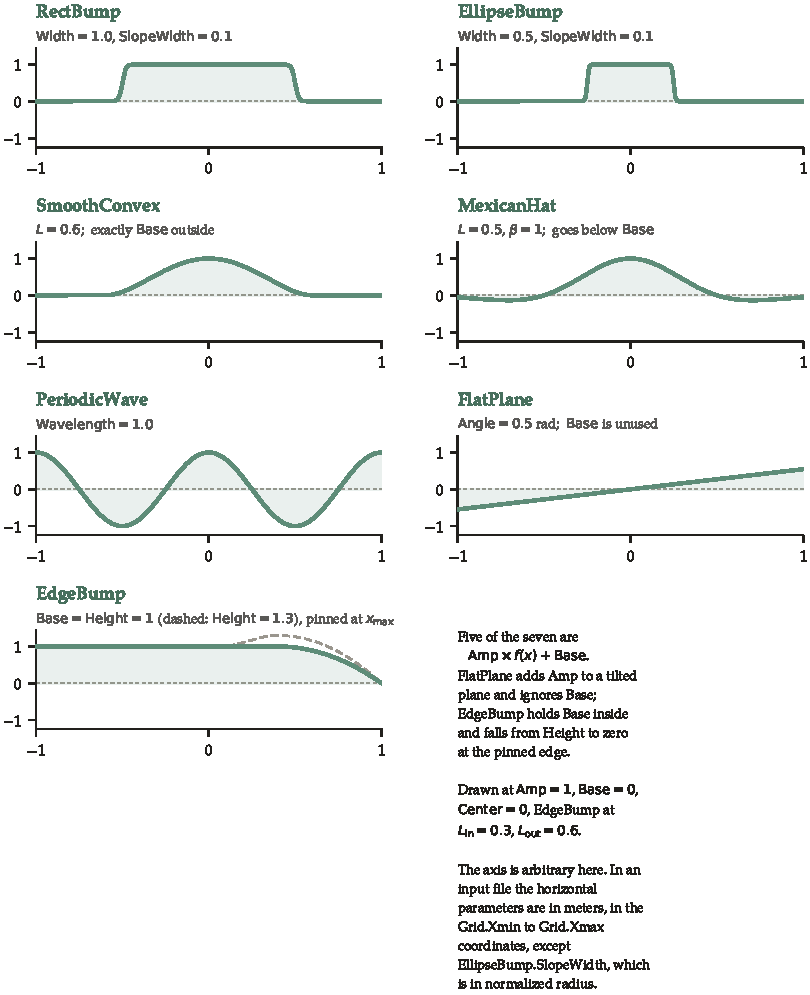
\includegraphics[width=\textwidth]{figures/shapes-1d.pdf}
  \caption{七つの形状関数。いずれも1次元で、$\mathrm{Amp}=1$、$\mathrm{Base}=0$、
    $\mathrm{Center}=0$として描いた。ただし\key{EdgeBump}は本来の使い方に合わせ、
    $\mathrm{Base}=\mathrm{Height}=1$の平坦な膜を$x_{\max}$で固定した形で描いた。
    五つの形状は$\mathrm{Amp}\times f + \mathrm{Base}$で評価する。
    $\mathrm{Amp}$はブロックの\key{Height}（\key{PeriodicWave}では
    \key{Amplitude}）、$f$は図の曲線であり、どちらも入れ物の
    \key{TotalHeight}に掛ける無次元の倍率である。残る二つは評価の仕方が異なる。
    \key{FlatPlane}は傾いた平面に$\mathrm{Amp}$を\emph{加え}、\key{Base}は一切
    使わない。\key{EdgeBump}は内側で\key{Base}を保ち、縁で\key{Height}からゼロまで
    下がる。図の横軸の目盛りは任意である。入力ファイルでは、\key{Center}、\key{Width}、
    \key{Wavelength}、\key{Phase}、\key{InnerLength}、\key{OuterLength}はメートル
    単位で、\key{Grid.Xmin}、\key{Grid.Xmax}と同じ座標系をとる。一方、
    \key{EllipseBump}の\key{SlopeWidth}は正規化半径を単位とする。
    \key{EdgeBump}の$r_s$は入力キーではなく、計算領域の縁から
    $x_{\max}-\key{OuterLength}$として求める。図もそのように描いた。
    \file{yuzen/src/\bk commonFunctions/\bk ShapeFunctions.cpp}の定義から
    \file{docs/manual/\bk figures/\bk make\_shapes.py}で作成した。
    \label{fig:shapes-1d}}
\end{figure}

\subsection{形状の組み合わせ方}
\label{sec:ref-domain:createtype}

一つの入れ物に属する形状は、すべて\key{Order}の昇順に並べ替える（同順位のものは
ファイル内の順序を保つ）。そのうえで、\textbf{ゼロから始まる}累積値に先頭から順に適用する。

\begin{description}
  \item[\val{"add"}] $\text{value} \leftarrow \max(\text{value}, \text{shape})$。
和ではなく\emph{和集合}をとる。
  \item[\val{"remove"}] $\text{value} \leftarrow \min(\text{value}, \text{shape})$。
  \item[\val{"stack"}] $\text{value} \leftarrow \text{value} + \text{shape}$。
\end{description}

\begin{warn}[\val{"add"}は加算ではなく最大値である]
  高さ\val{0.5}の隆起二つが重なっているとき、\val{"add"}で組み合わせると、重なった部分の高さは\val{1.0}
  ではなく\val{0.5}になる。足し合わせるのは\val{"stack"}だけである。既定値が
  \val{"add"}なので、\key{CreateType}を設定せずに複数の形状を並べると、それらの
  包絡になる。形状を横に並べるには\val{"add"}を、既存の形から輪郭を削り出すには
  \val{"remove"}（最小値）を、重ね合わせる（たとえば大きなドームに小さなさざ波を
  載せる）には\val{"stack"}を使う。
\end{warn}

重なり合う同じ二つのドームに三つの規則を適用した結果を\Cref{fig:shapes-createtype}に
示す。

\begin{figure}[tbp]
  \centering
  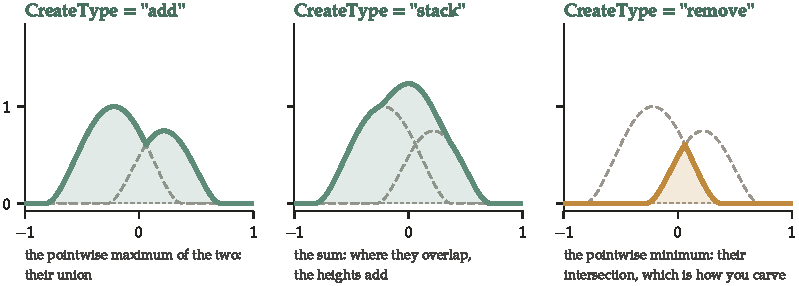
\includegraphics[width=\textwidth]{figures/shapes-createtype.pdf}
  \caption{\key{CreateType}の三つの合成規則を、重なり合う同じ二つの
    \key{SmoothConvex}形状（破線）に適用した結果。累積値はゼロから始まり、各形状を
    \key{Order}の順に取り込む。\val{"add"}は各点の\emph{最大値}をとるので、
    和ではなく和集合になる。\val{"stack"}は\emph{和}をとるので、重なった部分の高さは
    足し合わされる。\val{"remove"}は各点の\emph{最小値}をとり、既存の形から輪郭を
    削り出すのに使う。累積値はゼロから始まるので、何も加えないうちに\val{"remove"}で
    合成すると、その形状が正の値をとる場所には何も残らない。
    \label{fig:shapes-createtype}}
\end{figure}

水平方向の量（\key{Center}、\key{Width}、\key{Wavelength}、\key{Phase}、
\key{InnerLength}、\key{OuterLength}、\key{RectBump}の\key{SlopeWidth}）は、
\key{LengthScaleType}によらずメートル単位であり、\key{Grid.Xmin}、\key{Grid.Xmax}と
同じ座標系をとる。例外は\key{EllipseBump}の\key{SlopeWidth}である。正規化半径を
単位として縁をなまらせるので、無次元となる。鉛直方向の量（\key{Base}、
\key{Height}、\key{Amplitude}）は、入れ物の\key{TotalHeight}に掛ける無次元の倍率である。
\key{Center}、\key{Width}、\key{Wavelength}、\key{Phase}、\key{Angle}はいずれも配列で、
1次元の計算でも長さはちょうど~2とする。1次元の液膜は、形状を定義する平面上の
直線$y = 0$にあたるので、$y$成分も結果に影響する。同梱のケースはすべて\key{Center}と
\key{Phase}の$y$成分を0としており、この場合は各形状が$x$のキーどおりの分布を与える。しかし、
中心と$y = 0$の距離が$y$方向の広がりより大きい隆起は何も寄与しない。また、$y$方向に傾けた
\key{FlatPlane}では$-\mathrm{Center}_y \tan \mathrm{Angle}_y$が加わる。

\subsection{\key{Initial.SurfaceShape.RectBump}}

水準\key{Base}の上に高さ\key{Height}の矩形を立てた形状である。分布が微分可能になるよう、縁を
シグモイドでなまらせてある（\cref{fig:shapes-1d}の最初のパネル）。なまらせることで、
膜厚の方程式に現れる四階微分が角でも有限に保たれる。

\begin{keytable}{\key{RectBump}のキー（\key{Initial.SurfaceShape}または\key{Substrate}内）\label{tab:shape-rectbump}}\key{Order} & int & \val{0} & 並べ替えのキー。形状は昇順に適用する。任意の値。 \\
\key{CreateType} & string & \val{"add"} & 合成規則：\val{"add"}、\val{"remove"}、\val{"stack"}のいずれか。 \\
\key{Base} & double & \val{0} & 形状全体に加えるオフセット。\key{TotalHeight}に対する比。 \\
\key{Height} & double & \val{1} & 隆起の振幅。\key{TotalHeight}に対する比。 \\
\key{Center} & array & \val{[0, 0]} & 矩形の中心$(x,y)$（メートル）。長さはちょうど~2。 \\
\key{Width} & array & \val{[1, 1]} & 平坦な頂部の全幅$(x,y)$（メートル）。正。長さはちょうど~2。 \\
\key{SlopeWidth} & array & \val{[0.05, 0.05]} & 縁をなまらせる長さ$(x,y)$（メートル）。内部で0.1倍してシグモイドの幅とする。長さはちょうど~2。 \\
\end{keytable}

\subsection{\key{Initial.SurfaceShape.EllipseBump}}

楕円形の隆起であり、頂部が平らで縁がなめらかな台地状の形をとる（断面を\cref{fig:shapes-1d}の2番目のパネルに示す）。
台は$\sqrt{((x-c_x)/W_x)^2 + ((y-c_y)/W_y)^2} < 0.5$の内部なので、
\key{Width}は半軸長ではなく\emph{全}軸長である。同梱のケースで使っている形状はこれだけである。

\begin{keytable}{\key{EllipseBump}のキー（\key{Initial.SurfaceShape}または\key{Substrate}内）\label{tab:shape-ellipsebump}}\key{Order} & int & \val{0} & 並べ替えのキー。 \\
\key{CreateType} & string & \val{"add"} & 合成規則：\val{"add"}、\val{"remove"}、\val{"stack"}のいずれか。 \\
\key{Base} & double & \val{0} & 鉛直方向のオフセット。\key{TotalHeight}に対する比。 \\
\key{Height} & double & \val{1} & 振幅。\key{TotalHeight}に対する比。 \\
\key{Center} & array & \val{[0, 0]} & 中心$(x,y)$（メートル）。長さはちょうど~2。 \\
\key{Width} & array & \val{[1, 1]} & 全軸長$(x,y)$（メートル）。非ゼロ。長さはちょうど~2。 \\
\key{SlopeWidth} & double & \val{0.05} & 楕円の縁のなまらせ幅。正規化半径を単位とする。\key{RectBump}と違い\textbf{スカラー}である。 \\
\end{keytable}

\begin{warn}[縁の実際の幅をセル数で見積もること]
  ここでの\key{SlopeWidth}は\emph{正規化}半径に掛かるので、実空間での縁の幅は
  \key{Width}にも依存する。分布が\key{Height}の十分の一から十分の九まで変化する幅は
  \begin{equation*}
    \Delta x \;=\; \tfrac{1}{10}\ln 81 \;\key{SlopeWidth}\,W_x
              \;\approx\; 0.44\,\key{SlopeWidth}\,W_x ,
  \end{equation*}
  であり、重要なのはこの幅とセル幅$(X_{\max}-X_{\min})/N_x$との比である。既定値
  \val{0.05}は、\SI{0.4}{\milli\metre}の隆起では\SI{8.8}{\micro\metre}となり、1ミリメートルを
  60点で分割した格子の半セルにすぎない。\textbf{典型的な格子では、既定値のままだと段差になる}。
  長さのつもりで書いた値（たとえば\val{0.1e-3}）では垂直な壁になる。壁は見た目が
  悪いだけでは済まない。\file{concz\_2d}では、時間刻みが10分の1になり、隅に偽の液の
  膨らみが生じ（膜厚が\SI{6.05}{\micro\metre}のところ\SI{7.92}{\micro\metre}）、濃度の
  表面過剰量が2.7倍に膨らむ。縁が数セルにわたるよう設定し、長い計算の結果を信用する前に最初の
  \file{field00000.dat}を確認する必要がある。
\end{warn}

\subsection{\key{Initial.SurfaceShape.PeriodicWave}}

平均水準\key{Base}のまわりで振動する余弦の積である。
\[
  \text{shape} = \mathrm{Base} + \mathrm{Amplitude}\,
    \cos\!\left(\frac{2\pi (x-x_0)}{\lambda_x}\right)
    \cos\!\left(\frac{2\pi (y-y_0)}{\lambda_y}\right),
\]
波板状の基板や、単一波長のレベリング試験に使える。局在しない唯一の形状であり、
計算領域全体に広がって、\key{Base}の上下に同じだけ振れる（\cref{fig:shapes-1d}）。

\begin{keytable}{\key{PeriodicWave}のキー（\key{Initial.SurfaceShape}または\key{Substrate}内）\label{tab:shape-periodicwave}}\key{Order} & int & \val{0} & 並べ替えのキー。 \\
\key{CreateType} & string & \val{"add"} & 合成規則：\val{"add"}、\val{"remove"}、\val{"stack"}のいずれか。 \\
\key{Base} & double & \val{0} & 波の平均水準。\key{TotalHeight}に対する比。 \\
\key{Amplitude} & double & \val{1} & 振幅。\key{TotalHeight}に対する比。 \\
\key{Wavelength} & array & \val{[1, 1]} & 波長$(\lambda_x,\lambda_y)$（メートル）。非ゼロ。長さはちょうど~2。 \\
\key{Phase} & array & \val{[0, 0]} & 位相。角度ではなく\textbf{空間的なずれ}$(x_0,y_0)$（メートル）で与える。長さはちょうど~2。 \\
\end{keytable}

\subsection{\key{Initial.SurfaceShape.FlatPlane}}

次の傾いた平面である。
\[
  \text{shape} = (x-c_x)\tan\alpha_x + (y-c_y)\tan\alpha_y + \mathrm{Height},
\]
\key{Center}で高さ\key{Height}をとり、そこから一定の勾配で傾く
（\cref{fig:shapes-1d}）。\val{"stack"}と組み合わせれば、任意の形状に一様な
くさびを加えられる。

\begin{keytable}{\key{FlatPlane}のキー（\key{Initial.SurfaceShape}または\key{Substrate}内）\label{tab:shape-flatplane}}\key{Order} & int & \val{0} & 並べ替えのキー。 \\
\key{CreateType} & string & \val{"add"} & 合成規則：\val{"add"}、\val{"remove"}、\val{"stack"}のいずれか。 \\
\key{Height} & double & \val{1} & \key{Center}での平面の高さ。\key{TotalHeight}に対する比。 \\
\key{Center} & array & \val{[0, 0]} & 平面を傾ける支点$(x,y)$（メートル）。長さはちょうど~2。 \\
\key{Angle} & array & \val{[0, 0]} & $x$および$y$まわりの傾き。単位は\textbf{ラジアン}。長さはちょうど~2。 \\
\end{keytable}

\key{FlatPlane}には\key{Base}キーが\textbf{ない}。コンストラクターは常に基準値を
ゼロとして呼び出される。このキーを書いても効果はなく、警告も出ない。

\begin{warn}[ファイル中の二つの角度は単位が異なる]
  \key{FlatPlane.Angle}の単位は、入力ファイル中のほかの角度と同じくラジアンである。
  唯一の例外は\key{Physics.DisjoiningPressure.ContactAngle}で、単位は\emph{度}であり、
  $[0:90]$の範囲で検査する。したがって、接触角を\val{0.17}と書くと$10^\circ$
  ではなく六分の一度になる。
\end{warn}

\subsection{\key{Initial.SurfaceShape.MexicanHat}}

リッカーウェーブレット、つまり中央の山を円形の谷が囲む形である。ほかの局在した形状と
異なり、山のまわりで\key{Base}より\emph{下}に沈み、\key{Base}まで完全には戻らない。
このことは\cref{fig:shapes-1d}から一目で読み取れる。
\[
  \text{shape} = \mathrm{Base} + \mathrm{Height}\,(1-r^2)\,e^{-\beta r^2},
  \qquad
  r^2 = \left(\frac{x-c_x}{L_x}\right)^{2} + \left(\frac{y-c_y}{L_y}\right)^{2}.
\]

\begin{keytable}{\key{MexicanHat}のキー（\key{Initial.SurfaceShape}または\key{Substrate}内）\label{tab:shape-mexicanhat}}\key{Order} & int & \val{0} & 並べ替えのキー。 \\
\key{CreateType} & string & \val{"add"} & 合成規則：\val{"add"}、\val{"remove"}、\val{"stack"}のいずれか。 \\
\key{Base} & double & \val{0} & 鉛直方向のオフセット。\key{TotalHeight}に対する比。 \\
\key{Height} & double & \val{1} & 振幅。\key{TotalHeight}に対する比。 \\
\key{Center} & array & \val{[0, 0]} & 中心$(x,y)$（メートル）。長さはちょうど~2。 \\
\key{Width} & array & \val{[1, 1]} & 半径方向のスケール$(L_x,L_y)$（メートル）。長さはちょうど~2。成分がゼロだと、形状は至るところでゼロになる。 \\
\key{Beta} & double & \val{1} & ガウス包絡線の減衰率$\beta$。無次元。実用上は非負。 \\
\end{keytable}

\subsection{\key{Initial.SurfaceShape.SmoothConvex}}

コンパクトな台をもつドームであり、$r\le 1$の内部では$\mathrm{Height}\,(1-r^2)^2$、外部では
厳密に\key{Base}となる。$r$の定義は\key{MexicanHat}と同じである。楕円体と違って周囲の
水準に勾配ゼロで接するので、縁で曲率が突出しない。\cref{fig:shapes-1d}で、肩の形を
\key{MexicanHat}と比較されたい。

\begin{keytable}{\key{SmoothConvex}のキー（\key{Initial.SurfaceShape}または\key{Substrate}内）\label{tab:shape-smoothconvex}}\key{Order} & int & \val{0} & 並べ替えのキー。 \\
\key{CreateType} & string & \val{"add"} & 合成規則：\val{"add"}、\val{"remove"}、\val{"stack"}のいずれか。 \\
\key{Base} & double & \val{0} & 台の外側の水準。$r>1$ではこの値をそのまま返す。\key{TotalHeight}に対する比。 \\
\key{Height} & double & \val{1} & 頂点の振幅。\key{TotalHeight}に対する比。 \\
\key{Center} & array & \val{[0, 0]} & 中心$(x,y)$（メートル）。長さはちょうど~2。 \\
\key{Width} & array & \val{[1, 1]} & 半径方向の半幅$(L_x,L_y)$（メートル）。非ゼロ。長さはちょうど~2。 \\
\end{keytable}

\subsection{\key{Initial.SurfaceShape.EdgeBump}}

固定された縁に接する液膜を表す。計算領域の内側では\key{Base}の高さで平坦であり、縁の手前
\key{OuterLength}の区間でゼロまで下がる（\cref{fig:shapes-1d}の最後の
パネル）。不連続な状態からではなく、壁で固定されてメニスカスをもつ液膜から計算を
始めるための形状である。縁から\key{OuterLength}だけ内側にある切り替え点$r_s$からの
距離を$p$（縁に向かって正）とすると、分布は次式で与えられる。
%
\begin{equation}
  f(p) = \bigl(1-\sigma(p)\bigr)\Bigl[(H-B)\,\bigl(1-p^2/L_i^2\bigr)\,e^{-p^2/(\alpha L_i^2)} + B\Bigr]
       + \sigma(p)\,H\,\bigl(1 - p^2/L_o^2\bigr),
\end{equation}
%
ここで$B$ = \key{Base}、$H$ = \key{Height}、$L_i$ = \key{InnerLength}、$L_o$ =
\key{OuterLength}、$\alpha$ = \key{Alpha}であり、$\sigma$は$r_s$を中心とする幅
$0.1\,L_i$のロジスティック階段関数である。\textbf{通常は$\mathrm{Height} =
\mathrm{Base}$とする}（一様な厚さの液膜ならどちらも1）。このとき液膜は$r_s$まで平坦で、
縁に向かって放物線状にゼロまで下がる。\key{Height}を\key{Base}より大きくすると$r_s$に盛り上がり
（図の破線）ができ、小さくするとくぼみができる。

\textbf{\key{EdgeBump}を書けるのは\key{Initial.SurfaceShape}の中だけである}。\key{Substrate}
ブロックでは受け付けない。

\begin{keytable}{\key{Initial.SurfaceShape.EdgeBump}のキー\label{tab:shape-edgebump}}\key{Order} & int & \val{0} & 並べ替えのキー。 \\
\key{CreateType} & string & \val{"add"} & 合成規則：\val{"add"}、\val{"remove"}、\val{"stack"}のいずれか。 \\
\key{Base} & double & \val{0} & 縁から離れた計算領域内側での液膜の水準。\key{TotalHeight}に対する比。 \\
\key{Height} & double & \val{1} & 縁から\key{OuterLength}だけ内側にある切り替え点での水準。液膜はここから縁に向かってゼロまで下がる。メニスカスまで平坦な液膜にするには\key{Base}と同じ値にする。 \\
\key{Location} & string & \val{"Xmax"} & 隆起を付ける計算領域の縁。\val{"Xmin"}、\val{"Xmax"}、\val{"Ymin"}、\val{"Ymax"}のいずれか。対応する\key{Boundary}ブロックは\val{"Pinning"}型とする必要がある。 \\
\key{Alpha} & double & \val{1} & 内側のガウス関数$\exp(-(1/\alpha)(p/\mathrm{InnerLength})^2)$の幅パラメーター$\alpha>0$。無次元。 \\
\key{InnerLength} & double & \val{1} & 内側の長さスケール（メートル）。正。混合幅$0.1\,\mathrm{InnerLength}$もこの値で決まる。 \\
\key{OuterLength} & double & \val{1} & メニスカスの幅（メートル）。縁から切り替え点までの距離であり、この区間で液膜はゼロまで下がる。 \\
\end{keytable}

縁を固定する場合、液膜はその縁でゼロに達している必要がある。そうした液膜を与える形状が\key{EdgeBump}
である。分布は\key{Base}と\key{Height}の値によらず壁でゼロまで下がり、
\key{PrecursorRatio}が小さければ壁には前駆膜だけが残る。ソルバーは最初のステップの前にこの結果を
検査する（\cref{sec:ref-bcout:boundary}）。

\begin{note}[\key{Location}と境界条件は一致させること]
  各\key{EdgeBump}に対応する\key{Boundary.<Location>BC.Type}が\val{"Pinning"}でなければ、
  \code{CheckParameters}がメッセージ\code{Input mismatch}を出して入力を拒否する。
  これは、モデルを構築する前に検査するキー間の制約の一つである。液膜が固定した縁で
  実際にゼロに達しているかどうかは、最初のステップの直前に検査する（\cref{sec:ref-bcout:boundary}）。
\end{note}

\section{\key{Substrate}}
\label{sec:ref-domain:substrate}

\key{Substrate}は省略でき、書く場合も一回までである。このブロックでは、液膜が載る固体表面$s(x,y)$を
記述する。基板は動かず、形も変わらない。基板は自由表面の高さ$h+s$を通じて毛管圧の項と
鉛直重力の項に現れる。そのため、\textbf{この二つの項がどちらも無効なら、基板形状は
何の効果ももたない}（\cref{sec:terms:laplace,sec:terms:vgravity}）。

このブロックがなければ基板は平坦とみなす。形状は登録せず、分布も評価しない。

\begin{keytable}{\key{Substrate}のキー\label{tab:substrate-keys}}\key{TotalHeight} & double & \val{1} & 基板形状の高さスケール（メートル）。分布は合成した形状に\key{TotalHeight}を掛けたものになる。\key{Initial.SurfaceShape.TotalHeight}とは独立。 \\
\end{keytable}

\key{Substrate}では、\textbf{\key{EdgeBump}以外は}\key{Initial.SurfaceShape}と同じ
形状ブロックを繰り返し使える。\key{RectBump}、\key{EllipseBump}、
\key{PeriodicWave}、\key{FlatPlane}、\key{MexicanHat}、\key{SmoothConvex}の六つであり、
キー名、型、既定値、範囲、単位も同じである。二つのパーサーは書き込み先が違うだけで
コードは共通なので、\cref{tab:shape-rectbump,tab:shape-ellipsebump,tab:shape-periodicwave,tab:shape-flatplane,tab:shape-mexicanhat,tab:shape-smoothconvex}が
そのまま当てはまる。ほかに違うのは、\key{Base}、\key{Height}、\key{Amplitude}が
\key{Substrate.TotalHeight}に対する比になる点だけである。

\begin{note}[基板形状の並べ替えは試験していない]
  \file{cases/}には、\key{Substrate}の形状ブロック内で\key{Order}を設定したケースも、
  \key{EllipseBump}以外の基板形状を使うケースもない。複数の形状から基板を
  組み立てる場合は、結果を信用する前に最初の場の出力で形を確認する必要がある。
\end{note}

\section{\key{Fluid}}
\label{sec:ref-domain:fluid}

\key{Fluid}は必須で、ちょうど一回だけ書く。このブロック自身のキーが一つと、サブブロックが五つ
ある。サブブロック内のキーにはすべて既定値があるが、サブブロック自体は
\textbf{すべて必須}であり、一つでも欠けると計算を中止する。

\begin{keytable}{\key{Fluid}のキー\label{tab:fluid-keys}}\key{Name} & string & \val{"CR-EX"} & 液体の名前。記録してログに出力するだけであり、物性値の組を選ぶものではない。 \\
\end{keytable}

\subsection{濃度依存性}
\label{sec:ref-domain:fluidconc}

五つのサブブロックのうち三つでは、基準濃度での物性値と、その近くでの変化の仕方を与える。
\key{BaseValue}、\key{BaseConc}、\key{Coef}、\key{Exponent}の各キーは、次の三つの
法則の係数である。

\begin{align}
  \sigma(c) &= \mathrm{BaseValue} + \mathrm{Coef}\,(c - \mathrm{BaseConc}),
    \label{eq:fluid-sigma}\\
  \mu(c)    &= \mathrm{BaseValue}\,
    \exp\bigl(\mathrm{Exponent}\,(c - \mathrm{BaseConc})\bigr),
    \label{eq:fluid-mu}\\
  D(c)      &= \mathrm{BaseValue}\,
    \exp\bigl(\mathrm{Exponent}\,(c - \mathrm{BaseConc})\bigr).
    \label{eq:fluid-diff}
\end{align}

表面張力は濃度に対して線形に、粘度と拡散係数は指数関数的に変化する。ソルバーの中で
最も強い非線形性は\Cref{eq:fluid-mu}である。\key{Exponent}が10程度なら、濃度が0.1変化すると
粘度は$e$倍になる。液膜が乾くにつれて流れが止まるのは、この効果による。
\Cref{eq:fluid-sigma}は二か所に影響する。勾配\key{Coef}はマランゴニ数$\Ma$に
あたる。さらに$\sigma(c)$は毛管圧の項の移動度にも現れるので、乾燥が進むと液膜のレベリングの
速さも変わる（\cref{ch:concentration}）。

\subsection{\key{Fluid.Density}}

\begin{keytable}{\key{Fluid.Density}のキー\label{tab:fluid-density-keys}}\key{Value} & double & \val{1070} & 液体の密度$\rho$（\si{\kilogram\per\metre\cubed}）。正。濃度には依存しないと仮定する。毛管長$L_0$と、無次元数$\Bo$、$\Pvec$、$\Spn$に現れる。 \\
\end{keytable}

\subsection{\key{Fluid.SurfaceTension}}

\begin{keytable}{\key{Fluid.SurfaceTension}のキー（\cref{eq:fluid-sigma}を参照）\label{tab:fluid-surften-keys}}\key{BaseValue} & double & \val{0.028} & \key{BaseConc}での表面張力$\sigma_0$（\si{\newton\per\metre}）。正。毛管長と時間スケールがこの値で決まる。 \\
\key{BaseConc} & double & \val{0.5} & 線形則の基準濃度。質量分率で$[0:1]$。 \\
\key{Coef} & double & \val{0.014} & $\mathrm{d}\sigma/\mathrm{d}c$（単位濃度あたりの\si{\newton\per\metre}）。符号に意味がある。\key{BaseValue}との比がマランゴニ数$\Ma$になる。\key{Physics.SolutoCapillarity.Enable}が偽のときは強制的にゼロとする。 \\
\end{keytable}

\subsection{\key{Fluid.Viscosity}}

\begin{keytable}{\key{Fluid.Viscosity}のキー（\cref{eq:fluid-mu}を参照）\label{tab:fluid-visc-keys}}\key{BaseValue} & double & \val{0.115} & \key{BaseConc}での粘度$\mu_0$（\si{\pascal\second}）。正。時間スケール$T_0 = \mu_0 L_0^4/(\sigma_0 h_0^3)$がこの値で決まる。 \\
\key{BaseConc} & double & \val{0.5} & 基準濃度。質量分率で$[0:1]$。 \\
\key{Exponent} & double & \val{8} & 指数の係数。無次元で、任意の値。現実的な値は約10であり、このとき$\Delta c = 0.1$で$\mu$が$e$倍になる。 \\
\end{keytable}

\subsection{\key{Fluid.Diffusivity}}

\begin{keytable}{\key{Fluid.Diffusivity}のキー（\cref{eq:fluid-diff}を参照）\label{tab:fluid-diff-keys}}\key{BaseValue} & double & \val{9.78e-11} & \key{BaseConc}での溶質の拡散係数$D_0$（\si{\metre\squared\per\second}）。正。$\Pen = E_0 h_0/D_0$と$\Df = D_0 T_0/L_0^2$に現れる。 \\
\key{BaseConc} & double & \val{0.5} & 基準濃度。質量分率で$[0:1]$。 \\
\key{Exponent} & double & \val{6.94} & 指数の係数。無次元で、任意の値。実用上はふつう負である。 \\
\end{keytable}

\subsection{\key{Fluid.MolarMass}}

使うのは比$\Mr = \mathrm{Resin}/\mathrm{Solvent}$だけであり、この比は蒸発速度を与えるラウールの
法則に現れる（\cref{sec:terms:evaporation}）。したがって、両者の単位が揃っていれば単位は何でも
よい。

\begin{keytable}{\key{Fluid.MolarMass}のキー\label{tab:fluid-molar-keys}}\key{Solvent} & double & \val{106} & 溶媒のモル質量。正。通常は\si{\gram\per\mole}を用いるが、\key{Resin}と揃っていればどの単位でもよい。 \\
\key{Resin} & double & \val{2200} & 溶質のモル質量。正。\key{Solvent}と同じ単位。 \\
\end{keytable}
